\section{套利定理}
\begin{enumerate}[label=\arabic{section}.\arabic*]
    \item \sol\\
    不存在. 因为$\displaystyle p_i=\frac{1}{1+o_i}$,即
    \[p_1=\frac{1}{2},p_2=\frac{1}{3},p_3=\frac{1}{6} \Rightarrow \sum_{i=1}^3 p_i=1,\]
    所以不存在一个稳赢的赌博策略.
    \item \sol \[\frac{1}{1+2}+\frac{1}{1+3}+\frac{1}{1+o_4}=1 \Rightarrow o_4=\frac{47}{13}.\]
    \item \sol
    \begin{enumerate}[label=\alph*)]
        \item \[\begin{cases}
            4p_1+8p_2-10p_3=0,\\6p_1+12p_2-16p_3=0,
        \end{cases} \Rightarrow \rank \left(\begin{array}{ccc}
            \begin{matrix}
                4 & 8 & -10\\6 & 12 & -16
            \end{matrix}
        \end{array}\right)=2 \Rightarrow \text{不存在满足条件的}p_i,\]
        所以存在套利.
        \item \[\begin{cases}
            6p_1-3p_2=0,\\-2p_1+6p_3=0,\\10p_1+10p_2+xp_3=0,
        \end{cases} \text{有解} \Rightarrow x=-90,p_1=0.3,p_2=0.6,p_3=0.1,\]
        所以没有套利时,$x=-90$.
    \end{enumerate}
    \item \sol\\
    不存在套利时,仍有$\displaystyle p_1=\frac{1}{2},p_2=\frac{1}{3},p_3=\frac{1}{6}$,则
    \[\begin{cases}
        o_{12}(p_1+p_2)-p_3=0,\\o_{23}(p_2+p_3)-p_1=0,\\o_{13}(p_1+p_3)-p_2=0
    \end{cases} \Rightarrow \begin{cases}
        o_{12}=\frac{1}{5}, \\ o_{23}=1, \\ o_{13}=\frac{1}{2}.
    \end{cases}\]
    \item \pro\\
    若结果是$j$,则
    \begin{align*}
        o_jx_j-\sum_{i \neq j}x_i & = o_jx_j-\sum_{i = 1}^m x_i+x_j=(1+o_j)x_j-\sum_{i = 1}^m x_i\\
        &=\frac{(1+o_j)(1+o_j)^{-1}-\sum\limits_{i=1}^m (1+o_i)^{-1}}{1-\sum\limits_{i=1}^m (1+o_i)^{-1}}=1
    \end{align*}
    \item \sol\\
    购买看跌期权的收益为
    \[\begin{cases}
        -P, & \text{价格为}200 \\ \displaystyle\frac{100}{1+r}-P, & \text{价格为}50
    \end{cases}\]
    则\[E(\text{收益})=p\times(-P)+(1-p)\times\left(\frac{100}{1+r}-P\right)=(1-p)\frac{100}{1+r}-P,\]
    所以$\displaystyle P=(1-p)\frac{100}{1+r}=\left(1-\frac{1+2r}{3}\right)\frac{100}{1+r}=\frac{200(1-r)}{3(1+r)}$.\\
    因为$\displaystyle S+P-C=\frac{K}{1+r} \Rightarrow C=S+P-\frac{K}{1+r}$,代入可验证其成立.
    \item \sol\\
    先计算$\displaystyle p=\frac{1+r-d}{u-d}=\frac{1-1/2}{2-1/2}=\frac{1}{3}$(其中$r=0$),则有
    \begin{figure}[H]
        \centering
        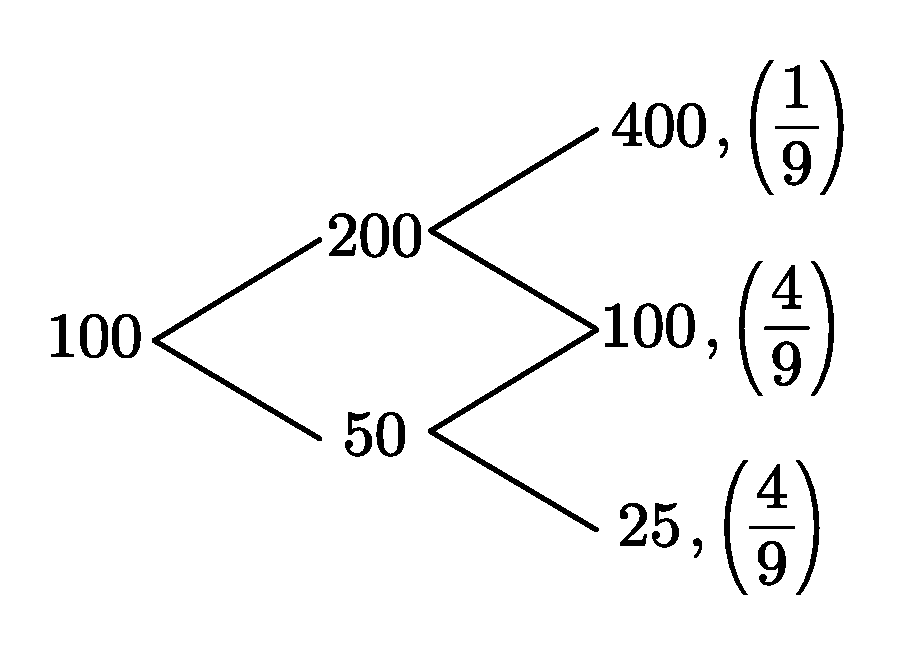
\includegraphics[scale=0.3]{6.7.pdf}
    \end{figure}
    所以收益为\[\begin{cases}
        \displaystyle\frac{250}{(1+r)^2}-C, & \text{概率为}1/9 \\ -C, & \text{概率为}4/9 \\ -C, & \text{概率为}4/9
    \end{cases}\]
    要使期望收益为0,则
    \[E(\text{收益})=\frac{250-C}{9}-\frac{4}{9}C-\frac{4}{9}C=0 \Rightarrow C=\frac{250}{9}.\]
    \item \sol {\kaishu \textcolor{blue}{注意:也可以参照教材例9.1a的解法.}}\\
    \begin{figure}[H]
        \centering
        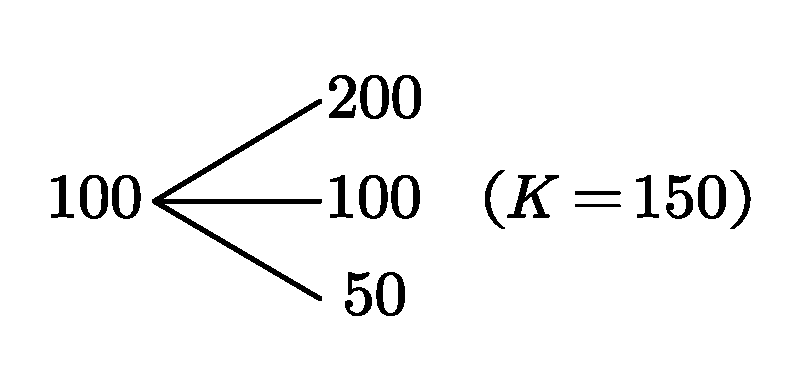
\includegraphics[scale=0.35]{6.8.pdf}
    \end{figure}
    买入股票的收益为
    \[\begin{cases}
        \displaystyle\frac{200}{1+r}-100, & \text{概率为}p_1 \\ \displaystyle\frac{100}{1+r}-100, & \text{概率为}p_2 \\ \displaystyle\frac{50}{1+r}-100, & \text{概率为}p_3 \\
    \end{cases}\]
    所以
    \[E(\text{买入股票的收益})=\left(\frac{200}{1+r}-100\right)p_1+\left(\frac{100}{1+r}-100\right)p_2+\left(\frac{50}{1+r}-100\right)p_3=0,\]
    买入期权的收益为$\displaystyle \begin{cases}
        \displaystyle\frac{50}{1+r}-C, & \text{概率为}p_1 \\ -C, & \text{概率为}p_2 \\ -C, & \text{概率为}p_3 \\
    \end{cases}$,所以\[E(\text{买入期权的收益})=\left(\frac{50}{1+r}-C\right)p_1-Cp_2-Cp_3=0,\]
    由后式可得$\displaystyle C=\frac{50p_1}{1+r}$,由前式可得
    \begin{align*}
        &\left(\frac{200}{1+r}\right)p_1+\left(\frac{100}{1+r}\right)p_2+\left(\frac{50}{1+r}\right)p_3=100(p_1+p_2+p_3)=100\\
        \Rightarrow & 2p_1+p_2+\frac{1}{2}p_3=1+r \Rightarrow 2p_1+p_2+\frac{1}{2}(1-p_1-p_2)=1+r\\
        \Rightarrow & 3p_1+p_2=1+2r \Rightarrow p_1=\frac{1+2r-p_2}{3}
    \end{align*}
    所以$\displaystyle C=\frac{50p_1}{1+r}=\frac{1+2r-p_2}{3}\cdot\frac{50}{1+r}$,由$0 \leq p_2 \leq 1$可得
    \[\frac{2r}{3}\cdot\frac{50}{1+r} \leq C \leq \frac{1+2r}{3}\cdot\frac{50}{1+r} \Rightarrow 0 \leq C \leq \frac{50}{3}.\]
    \item \sol
    \begin{enumerate}[label=\alph*)]
        \item 若$C=0$,则在时刻0,无支出;在时刻1可收入50或0,这显然是个弱套利.
        \item 若$\displaystyle C=\frac{50}{3}$,则在时刻0,卖出一个看涨期权,并买入$x$股股票;在时刻1,收入如下表:
        \begin{table}[H]
            \centering
            \begin{tabular}{|c|c|c|c|}
                \hline
                时刻1股票的价格 & 时刻0的余额 & 时刻1该投资的现值 & 收入$(r=0)$ \\ \hline
                200 & $50/3-100x$ & $-50+200x$ & $100x-100/3$ \\ \hline
                100 & $50/3-100x$ & $0+100x$ & $50/3$ \\ \hline
                50 & $50/3-100x$ & $0+50x$ & $-50x-100/3$ \\ \hline
            \end{tabular}
        \end{table}
        若$\displaystyle x=\frac{1}{3}$,则显然存在弱套利机会. 综上,弱套利可能存在.
    \end{enumerate}
    \item \sol\\
    令$S(0)=s$,假设$us>K>ds$. 如果通过借$x$来买入$y$份证券,则在时刻$t$,剩余$ys-x$的收入为
    \[\begin{cases}
        yus-(1+r)x, & S(1)=us\\yds-(1+r)x, & S(1)=ds
    \end{cases}\]
    所以可以通过如下方式复制期权,
    \[\begin{cases}
        yus-(1+r)x=us-K,\\yds-(1+r)x=0,
    \end{cases}\]
    令$\displaystyle y=\frac{us-K}{(u-d)s},x=\frac{ds(us-K)}{(1+r)(u-d)s}$,则根据一价律,期权的无套利价格是$\displaystyle ys-x=\frac{us-K}{u-d}-\frac{ds(us-K)}{(1+r)(u-d)s}$.
    \item \sol
    \begin{enumerate}[label=\alph*)]
        \item $\displaystyle p=\frac{1+r-d}{u-d}=\frac{0.3}{0.425}=\frac{12}{17}$,期望收益为$25(1-p)^2p^3=0.7606$,所以无套利价格是$0.7606\times 1.1^{-5}=0.4723$.
        \item 是唯一的. 证明略.
        \item $\displaystyle 25 \times \left(\frac{1}{2}\right)^5=0.78125$.
    \end{enumerate}
    \item \sol\\
    $\displaystyle p=\frac{1+r-d}{u-d}=0.7380$,如果前3个时刻中至少有2个时刻是向上的,则可得到回报,所以
    \[C=\e^{-0.05 \times 3}\times 100 \left[0.7380^3+3(0.7380)^2(1-0.7380)\right]=84.5228.\]
\end{enumerate}
\clearpage